\begin{figure}
\centering
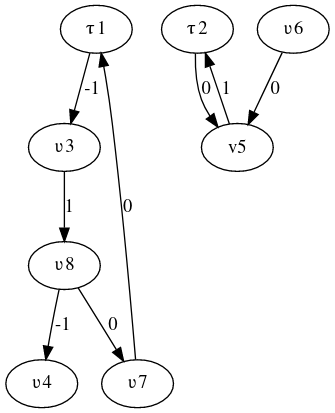
\includegraphics[width=0.3\linewidth]{figures/digraph.png}
% Generating the graph requires \usepackage{dot2texi} or \usepackage[pdf]{graphviz}
\iffalse
\begin{dot2tex}[file=cstrnts,scale=0.6]
digraph D {
    t1 [label=<&tau;<SUB>1</SUB>>];
    t2 [label=<&tau;<SUB>2</SUB>>];
    v3 [label=<&upsilon;<SUB>3</SUB>>];
    v4 [label=<&upsilon;<SUB>4</SUB>>];
    v6 [label=<&upsilon;<SUB>6</SUB>>];
    v7 [label=<&upsilon;<SUB>7</SUB>>];
    v8 [label=<&upsilon;<SUB>8</SUB>>];
    v7 -> t1 [label="0"];
    v8 -> v7 [label="0"];
    t2 -> v5 [label="0"];
    v6 -> v5 [label="0"];
    v8 -> v4 [label="-1"];
    v3 -> v8 [label="1"];
    t1 -> v3 [label="-1"];
    v5 -> t2 [label="1"];
}
\end{dot2tex}
\fi
\caption{Example size variable constraints as a weighted directed graph}
\label{fig:digraph}
\end{figure}
